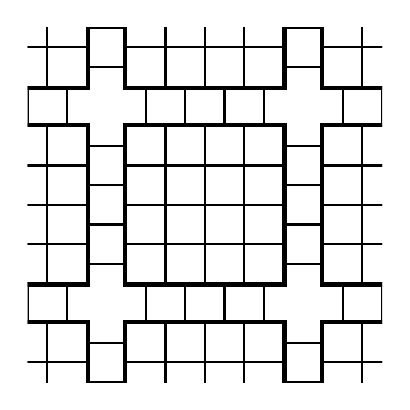
\begin{tikzpicture}[thick]
	\pgfmathsetmacro{\scale}{0.5}
	
	\pgfmathtruncatemacro{\width}{4}
	\pgfmathtruncatemacro{\height}{4}
	
	\begin{scope}[scale=\scale]
		\clip (-2, -2)
		      rectangle
		      (\width + 3.0, \height + 3.0);
		
		\foreach \xx in {-1,0,1}{
			\foreach \yy in {-1,0,1}{
				% Nodes in partition
				\foreach \x in {1,...,\width}{
					\foreach \y in {1,...,\height}{
						\pgfmathtruncatemacro{\posx}{((\width+1) * \xx) + \x}
						\pgfmathtruncatemacro{\posy}{((\height+1) * \yy) + \y}
						\node (node\xx\yy\x\y) at (\posx, \posy)
						      [ minimum width=\scale*1cm
						      , minimum height=\scale*1cm
						      , inner sep=0
						      , draw
						      , rectangle]
						      {};
					}
				}
				
				% Outline around partition
				\draw [ultra thick]
				      (node\xx\yy11.south west)
				      rectangle
				      (node\xx\yy\width\height.north east);
			}
		}
		
		% Links between partitions
		\foreach \xx in {-1,0,1}{
			\foreach \yy in {-1,0}{
				\foreach \x in {1,...,\width}{
					\pgfmathtruncatemacro{\destyy}{\yy+1}
					\draw (node\xx\yy\x\height) -- (node\xx\destyy\x1);
				}
			}
		}
		\foreach \xx in {-1,0}{
			\foreach \yy in {-1,0,1}{
				\foreach \y in {1,...,\height}{
					\pgfmathtruncatemacro{\destxx}{\xx+1}
					\draw (node\xx\yy\width\y) -- (node\destxx\yy1\y);
				}
			}
		}
	\end{scope}
	
\end{tikzpicture}

